\PassOptionsToPackage{unicode=true}{hyperref} % options for packages loaded elsewhere
\PassOptionsToPackage{hyphens}{url}
%
\documentclass[
]{article}
\usepackage{lmodern}
\usepackage{amssymb,amsmath}
\usepackage{ifxetex,ifluatex}
\ifnum 0\ifxetex 1\fi\ifluatex 1\fi=0 % if pdftex
  \usepackage[T1]{fontenc}
  \usepackage[utf8]{inputenc}
  \usepackage{textcomp} % provides euro and other symbols
\else % if luatex or xelatex
  \usepackage{unicode-math}
  \defaultfontfeatures{Scale=MatchLowercase}
  \defaultfontfeatures[\rmfamily]{Ligatures=TeX,Scale=1}
\fi
% use upquote if available, for straight quotes in verbatim environments
\IfFileExists{upquote.sty}{\usepackage{upquote}}{}
\IfFileExists{microtype.sty}{% use microtype if available
  \usepackage[]{microtype}
  \UseMicrotypeSet[protrusion]{basicmath} % disable protrusion for tt fonts
}{}
\makeatletter
\@ifundefined{KOMAClassName}{% if non-KOMA class
  \IfFileExists{parskip.sty}{%
    \usepackage{parskip}
  }{% else
    \setlength{\parindent}{0pt}
    \setlength{\parskip}{6pt plus 2pt minus 1pt}}
}{% if KOMA class
  \KOMAoptions{parskip=half}}
\makeatother
\usepackage{xcolor}
\IfFileExists{xurl.sty}{\usepackage{xurl}}{} % add URL line breaks if available
\IfFileExists{bookmark.sty}{\usepackage{bookmark}}{\usepackage{hyperref}}
\hypersetup{
  pdftitle={Notes for Atika},
  pdfauthor={Jonathan A. Pedroza},
  pdfborder={0 0 0},
  breaklinks=true}
\urlstyle{same}  % don't use monospace font for urls
\usepackage[margin=1in]{geometry}
\usepackage{color}
\usepackage{fancyvrb}
\newcommand{\VerbBar}{|}
\newcommand{\VERB}{\Verb[commandchars=\\\{\}]}
\DefineVerbatimEnvironment{Highlighting}{Verbatim}{commandchars=\\\{\}}
% Add ',fontsize=\small' for more characters per line
\usepackage{framed}
\definecolor{shadecolor}{RGB}{248,248,248}
\newenvironment{Shaded}{\begin{snugshade}}{\end{snugshade}}
\newcommand{\AlertTok}[1]{\textcolor[rgb]{0.94,0.16,0.16}{#1}}
\newcommand{\AnnotationTok}[1]{\textcolor[rgb]{0.56,0.35,0.01}{\textbf{\textit{#1}}}}
\newcommand{\AttributeTok}[1]{\textcolor[rgb]{0.77,0.63,0.00}{#1}}
\newcommand{\BaseNTok}[1]{\textcolor[rgb]{0.00,0.00,0.81}{#1}}
\newcommand{\BuiltInTok}[1]{#1}
\newcommand{\CharTok}[1]{\textcolor[rgb]{0.31,0.60,0.02}{#1}}
\newcommand{\CommentTok}[1]{\textcolor[rgb]{0.56,0.35,0.01}{\textit{#1}}}
\newcommand{\CommentVarTok}[1]{\textcolor[rgb]{0.56,0.35,0.01}{\textbf{\textit{#1}}}}
\newcommand{\ConstantTok}[1]{\textcolor[rgb]{0.00,0.00,0.00}{#1}}
\newcommand{\ControlFlowTok}[1]{\textcolor[rgb]{0.13,0.29,0.53}{\textbf{#1}}}
\newcommand{\DataTypeTok}[1]{\textcolor[rgb]{0.13,0.29,0.53}{#1}}
\newcommand{\DecValTok}[1]{\textcolor[rgb]{0.00,0.00,0.81}{#1}}
\newcommand{\DocumentationTok}[1]{\textcolor[rgb]{0.56,0.35,0.01}{\textbf{\textit{#1}}}}
\newcommand{\ErrorTok}[1]{\textcolor[rgb]{0.64,0.00,0.00}{\textbf{#1}}}
\newcommand{\ExtensionTok}[1]{#1}
\newcommand{\FloatTok}[1]{\textcolor[rgb]{0.00,0.00,0.81}{#1}}
\newcommand{\FunctionTok}[1]{\textcolor[rgb]{0.00,0.00,0.00}{#1}}
\newcommand{\ImportTok}[1]{#1}
\newcommand{\InformationTok}[1]{\textcolor[rgb]{0.56,0.35,0.01}{\textbf{\textit{#1}}}}
\newcommand{\KeywordTok}[1]{\textcolor[rgb]{0.13,0.29,0.53}{\textbf{#1}}}
\newcommand{\NormalTok}[1]{#1}
\newcommand{\OperatorTok}[1]{\textcolor[rgb]{0.81,0.36,0.00}{\textbf{#1}}}
\newcommand{\OtherTok}[1]{\textcolor[rgb]{0.56,0.35,0.01}{#1}}
\newcommand{\PreprocessorTok}[1]{\textcolor[rgb]{0.56,0.35,0.01}{\textit{#1}}}
\newcommand{\RegionMarkerTok}[1]{#1}
\newcommand{\SpecialCharTok}[1]{\textcolor[rgb]{0.00,0.00,0.00}{#1}}
\newcommand{\SpecialStringTok}[1]{\textcolor[rgb]{0.31,0.60,0.02}{#1}}
\newcommand{\StringTok}[1]{\textcolor[rgb]{0.31,0.60,0.02}{#1}}
\newcommand{\VariableTok}[1]{\textcolor[rgb]{0.00,0.00,0.00}{#1}}
\newcommand{\VerbatimStringTok}[1]{\textcolor[rgb]{0.31,0.60,0.02}{#1}}
\newcommand{\WarningTok}[1]{\textcolor[rgb]{0.56,0.35,0.01}{\textbf{\textit{#1}}}}
\usepackage{graphicx,grffile}
\makeatletter
\def\maxwidth{\ifdim\Gin@nat@width>\linewidth\linewidth\else\Gin@nat@width\fi}
\def\maxheight{\ifdim\Gin@nat@height>\textheight\textheight\else\Gin@nat@height\fi}
\makeatother
% Scale images if necessary, so that they will not overflow the page
% margins by default, and it is still possible to overwrite the defaults
% using explicit options in \includegraphics[width, height, ...]{}
\setkeys{Gin}{width=\maxwidth,height=\maxheight,keepaspectratio}
\setlength{\emergencystretch}{3em}  % prevent overfull lines
\providecommand{\tightlist}{%
  \setlength{\itemsep}{0pt}\setlength{\parskip}{0pt}}
\setcounter{secnumdepth}{-2}
% Redefines (sub)paragraphs to behave more like sections
\ifx\paragraph\undefined\else
  \let\oldparagraph\paragraph
  \renewcommand{\paragraph}[1]{\oldparagraph{#1}\mbox{}}
\fi
\ifx\subparagraph\undefined\else
  \let\oldsubparagraph\subparagraph
  \renewcommand{\subparagraph}[1]{\oldsubparagraph{#1}\mbox{}}
\fi

% set default figure placement to htbp
\makeatletter
\def\fps@figure{htbp}
\makeatother


\title{Notes for Atika}
\author{Jonathan A. Pedroza}
\date{4/17/2020}

\begin{document}
\maketitle

\hypertarget{data-manipulation-proposed-models}{%
\section{Data Manipulation \& Proposed
Models}\label{data-manipulation-proposed-models}}

\begin{Shaded}
\begin{Highlighting}[]
\KeywordTok{library}\NormalTok{(tidyverse)}
\end{Highlighting}
\end{Shaded}

\begin{verbatim}
## Warning: package 'tidyverse' was built under R version 3.6.3
\end{verbatim}

\begin{verbatim}
## -- Attaching packages ------------------------------------- tidyverse 1.3.0 --
\end{verbatim}

\begin{verbatim}
## v ggplot2 3.3.0     v purrr   0.3.3
## v tibble  2.1.3     v dplyr   0.8.3
## v tidyr   1.0.2     v stringr 1.4.0
## v readr   1.3.1     v forcats 0.4.0
\end{verbatim}

\begin{verbatim}
## Warning: package 'ggplot2' was built under R version 3.6.3
\end{verbatim}

\begin{verbatim}
## Warning: package 'purrr' was built under R version 3.6.3
\end{verbatim}

\begin{verbatim}
## -- Conflicts ---------------------------------------- tidyverse_conflicts() --
## x dplyr::filter() masks stats::filter()
## x dplyr::lag()    masks stats::lag()
\end{verbatim}

\begin{Shaded}
\begin{Highlighting}[]
\KeywordTok{library}\NormalTok{(inspectdf)}
\KeywordTok{library}\NormalTok{(psych)}
\end{Highlighting}
\end{Shaded}

\begin{verbatim}
## 
## Attaching package: 'psych'
\end{verbatim}

\begin{verbatim}
## The following objects are masked from 'package:ggplot2':
## 
##     %+%, alpha
\end{verbatim}

\begin{Shaded}
\begin{Highlighting}[]
\KeywordTok{library}\NormalTok{(lme4)}
\end{Highlighting}
\end{Shaded}

\begin{verbatim}
## Loading required package: Matrix
\end{verbatim}

\begin{verbatim}
## 
## Attaching package: 'Matrix'
\end{verbatim}

\begin{verbatim}
## The following objects are masked from 'package:tidyr':
## 
##     expand, pack, unpack
\end{verbatim}

\begin{Shaded}
\begin{Highlighting}[]
\KeywordTok{library}\NormalTok{(lmerTest)}
\end{Highlighting}
\end{Shaded}

\begin{verbatim}
## Warning: package 'lmerTest' was built under R version 3.6.2
\end{verbatim}

\begin{verbatim}
## 
## Attaching package: 'lmerTest'
\end{verbatim}

\begin{verbatim}
## The following object is masked from 'package:lme4':
## 
##     lmer
\end{verbatim}

\begin{verbatim}
## The following object is masked from 'package:stats':
## 
##     step
\end{verbatim}

\begin{Shaded}
\begin{Highlighting}[]
\KeywordTok{library}\NormalTok{(optimx)}
\end{Highlighting}
\end{Shaded}

\begin{verbatim}
## Warning: package 'optimx' was built under R version 3.6.2
\end{verbatim}

\begin{Shaded}
\begin{Highlighting}[]
\KeywordTok{options}\NormalTok{(}\DataTypeTok{max.print =} \DecValTok{99999}\NormalTok{)}
\KeywordTok{options}\NormalTok{(}\DataTypeTok{scipen =} \DecValTok{999}\NormalTok{)}
\KeywordTok{theme_set}\NormalTok{(}\KeywordTok{theme_minimal}\NormalTok{())}


\KeywordTok{getwd}\NormalTok{()}
\end{Highlighting}
\end{Shaded}

\begin{verbatim}
## [1] "C:/Users/cpppe/OneDrive/Desktop/github shared projects/dissertation/write-ups"
\end{verbatim}

\begin{Shaded}
\begin{Highlighting}[]
\KeywordTok{set.seed}\NormalTok{(}\DecValTok{04092020}\NormalTok{)}
\end{Highlighting}
\end{Shaded}

\begin{Shaded}
\begin{Highlighting}[]
\NormalTok{county16 <-}\StringTok{ }\KeywordTok{read_csv}\NormalTok{(}\StringTok{"C:/Users/cpppe/OneDrive/Desktop/github shared projects/dissertation/final_data/county16_sub.csv"}\NormalTok{)}
\end{Highlighting}
\end{Shaded}

\begin{verbatim}
## Warning: Missing column names filled in: 'X1' [1]
\end{verbatim}

\begin{verbatim}
## Parsed with column specification:
## cols(
##   .default = col_double(),
##   state_fips_code = col_character(),
##   county_fips_code = col_character(),
##   fips_code = col_character(),
##   state_abbreviation = col_character(),
##   county_name = col_character(),
##   communicable_disease = col_logical(),
##   coronary_heart_disease_hospitalizations = col_logical(),
##   cerebrovascular_disease_hospitalizations = col_logical(),
##   self_inflicted_injury_hospitalizations = col_logical(),
##   smoking_during_pregnancy = col_logical(),
##   drug_arrests = col_logical(),
##   alcohol_related_hospitalizations = col_logical(),
##   motor_vehicle_crash_occupancy_rate = col_logical(),
##   on_road_motor_vehicle_crash_related_er_visits = col_logical(),
##   off_road_motor_vehicle_crash_related_er_visits = col_logical(),
##   no_recent_dental_visit = col_logical(),
##   did_not_get_needed_health_care = col_logical(),
##   childhood_immunizations = col_logical(),
##   local_health_department_staffing = col_logical(),
##   reading_proficiency = col_logical()
##   # ... with 19 more columns
## )
\end{verbatim}

\begin{verbatim}
## See spec(...) for full column specifications.
\end{verbatim}

\begin{verbatim}
## Warning: 2341 parsing failures.
##  row                                      col           expected   actual                                                                                              file
## 3097 communicable_disease                     1/0/T/F/TRUE/FALSE 802.72   'C:/Users/cpppe/OneDrive/Desktop/github shared projects/dissertation/final_data/county16_sub.csv'
## 3097 coronary_heart_disease_hospitalizations  1/0/T/F/TRUE/FALSE 3.1      'C:/Users/cpppe/OneDrive/Desktop/github shared projects/dissertation/final_data/county16_sub.csv'
## 3097 cerebrovascular_disease_hospitalizations 1/0/T/F/TRUE/FALSE 2.5      'C:/Users/cpppe/OneDrive/Desktop/github shared projects/dissertation/final_data/county16_sub.csv'
## 3097 self_inflicted_injury_hospitalizations   1/0/T/F/TRUE/FALSE 96.4     'C:/Users/cpppe/OneDrive/Desktop/github shared projects/dissertation/final_data/county16_sub.csv'
## 3097 smoking_during_pregnancy                 1/0/T/F/TRUE/FALSE 0.138595 'C:/Users/cpppe/OneDrive/Desktop/github shared projects/dissertation/final_data/county16_sub.csv'
## .... ........................................ .................. ........ .................................................................................................
## See problems(...) for more details.
\end{verbatim}

\begin{Shaded}
\begin{Highlighting}[]
\NormalTok{county17 <-}\StringTok{ }\KeywordTok{read_csv}\NormalTok{(}\StringTok{"C:/Users/cpppe/OneDrive/Desktop/github shared projects/dissertation/final_data/county17_sub.csv"}\NormalTok{)}
\end{Highlighting}
\end{Shaded}

\begin{verbatim}
## Warning: Missing column names filled in: 'X1' [1]
\end{verbatim}

\begin{verbatim}
## Parsed with column specification:
## cols(
##   .default = col_double(),
##   state_fips_code = col_character(),
##   county_fips_code = col_character(),
##   fips_code = col_character(),
##   state_abbreviation = col_character(),
##   county_name = col_character(),
##   communicable_disease = col_logical(),
##   coronary_heart_disease_hospitalizations = col_logical(),
##   cerebrovascular_disease_hospitalizations = col_logical(),
##   self_inflicted_injury_hospitalizations = col_logical(),
##   cancer_incidence = col_logical(),
##   smoking_during_pregnancy = col_logical(),
##   drug_arrests = col_logical(),
##   alcohol_related_hospitalizations = col_logical(),
##   motor_vehicle_crash_occupancy_rate = col_logical(),
##   on_road_motor_vehicle_crash_related_er_visits = col_logical(),
##   off_road_motor_vehicle_crash_related_er_visits = col_logical(),
##   no_recent_dental_visit = col_logical(),
##   did_not_get_needed_health_care = col_logical(),
##   childhood_immunizations = col_logical(),
##   local_health_department_staffing = col_logical()
##   # ... with 20 more columns
## )
## See spec(...) for full column specifications.
\end{verbatim}

\begin{verbatim}
## Warning: 2416 parsing failures.
##  row                                      col           expected actual                                                                                              file
## 3093 communicable_disease                     1/0/T/F/TRUE/FALSE 838.68 'C:/Users/cpppe/OneDrive/Desktop/github shared projects/dissertation/final_data/county17_sub.csv'
## 3093 coronary_heart_disease_hospitalizations  1/0/T/F/TRUE/FALSE 2.8    'C:/Users/cpppe/OneDrive/Desktop/github shared projects/dissertation/final_data/county17_sub.csv'
## 3093 cerebrovascular_disease_hospitalizations 1/0/T/F/TRUE/FALSE 2.5    'C:/Users/cpppe/OneDrive/Desktop/github shared projects/dissertation/final_data/county17_sub.csv'
## 3093 self_inflicted_injury_hospitalizations   1/0/T/F/TRUE/FALSE 98.6   'C:/Users/cpppe/OneDrive/Desktop/github shared projects/dissertation/final_data/county17_sub.csv'
## 3093 cancer_incidence                         1/0/T/F/TRUE/FALSE 468.2  'C:/Users/cpppe/OneDrive/Desktop/github shared projects/dissertation/final_data/county17_sub.csv'
## .... ........................................ .................. ...... .................................................................................................
## See problems(...) for more details.
\end{verbatim}

\begin{Shaded}
\begin{Highlighting}[]
\NormalTok{county18 <-}\StringTok{ }\KeywordTok{read_csv}\NormalTok{(}\StringTok{"C:/Users/cpppe/OneDrive/Desktop/github shared projects/dissertation/final_data/county18_sub.csv"}\NormalTok{)}
\end{Highlighting}
\end{Shaded}

\begin{verbatim}
## Warning: Missing column names filled in: 'X1' [1]
\end{verbatim}

\begin{verbatim}
## Parsed with column specification:
## cols(
##   .default = col_double(),
##   state_fips_code = col_character(),
##   county_fips_code = col_character(),
##   fips_code = col_character(),
##   state_abbreviation = col_character(),
##   county_name = col_character(),
##   communicable_disease = col_logical(),
##   self_inflicted_injury_hospitalizations = col_logical(),
##   cancer_incidence = col_logical(),
##   smoking_during_pregnancy = col_logical(),
##   drug_arrests = col_logical(),
##   motor_vehicle_crash_occupancy_rate = col_logical(),
##   on_road_motor_vehicle_crash_related_er_visits = col_logical(),
##   off_road_motor_vehicle_crash_related_er_visits = col_logical(),
##   no_recent_dental_visit = col_logical(),
##   did_not_get_needed_health_care = col_logical(),
##   childhood_immunizations = col_logical(),
##   reading_proficiency = col_logical(),
##   w_2_enrollment = col_logical(),
##   poverty = col_logical(),
##   older_adults_living_alone = col_logical()
##   # ... with 16 more columns
## )
## See spec(...) for full column specifications.
\end{verbatim}

\begin{verbatim}
## Warning: 2142 parsing failures.
##  row                                    col           expected       actual                                                                                              file
## 3098 communicable_disease                   1/0/T/F/TRUE/FALSE 881.86       'C:/Users/cpppe/OneDrive/Desktop/github shared projects/dissertation/final_data/county18_sub.csv'
## 3098 self_inflicted_injury_hospitalizations 1/0/T/F/TRUE/FALSE 98.6         'C:/Users/cpppe/OneDrive/Desktop/github shared projects/dissertation/final_data/county18_sub.csv'
## 3098 cancer_incidence                       1/0/T/F/TRUE/FALSE 469.3        'C:/Users/cpppe/OneDrive/Desktop/github shared projects/dissertation/final_data/county18_sub.csv'
## 3098 smoking_during_pregnancy               1/0/T/F/TRUE/FALSE 0.1251113057 'C:/Users/cpppe/OneDrive/Desktop/github shared projects/dissertation/final_data/county18_sub.csv'
## 3098 drug_arrests                           1/0/T/F/TRUE/FALSE 25990        'C:/Users/cpppe/OneDrive/Desktop/github shared projects/dissertation/final_data/county18_sub.csv'
## .... ...................................... .................. ............ .................................................................................................
## See problems(...) for more details.
\end{verbatim}

\begin{Shaded}
\begin{Highlighting}[]
\NormalTok{county19 <-}\StringTok{ }\KeywordTok{read_csv}\NormalTok{(}\StringTok{"C:/Users/cpppe/OneDrive/Desktop/github shared projects/dissertation/final_data/county19_sub.csv"}\NormalTok{)}
\end{Highlighting}
\end{Shaded}

\begin{verbatim}
## Warning: Missing column names filled in: 'X1' [1]
\end{verbatim}

\begin{verbatim}
## Parsed with column specification:
## cols(
##   .default = col_double(),
##   state_fips_code = col_character(),
##   county_fips_code = col_character(),
##   fips_code = col_character(),
##   state_abbreviation = col_character(),
##   county_name = col_character(),
##   communicable_disease = col_logical(),
##   self_inflicted_injury_hospitalizations = col_logical(),
##   cancer_incidence = col_logical(),
##   coronary_heart_disease_hospitalizations = col_logical(),
##   cerebrovascular_disease_hospitalizations = col_logical(),
##   smoking_during_pregnancy = col_logical(),
##   drug_arrests = col_logical(),
##   opioid_hospital_visits = col_logical(),
##   alcohol_related_hospitalizations = col_logical(),
##   motor_vehicle_crash_occupancy_rate = col_logical(),
##   on_road_motor_vehicle_crash_related_er_visits = col_logical(),
##   off_road_motor_vehicle_crash_related_er_visits = col_logical(),
##   childhood_immunizations = col_logical(),
##   reading_proficiency = col_logical(),
##   w_2_enrollment = col_logical()
##   # ... with 18 more columns
## )
## See spec(...) for full column specifications.
\end{verbatim}

\begin{verbatim}
## Warning: 2316 parsing failures.
##  row                                      col           expected       actual                                                                                              file
## 3098 communicable_disease                     1/0/T/F/TRUE/FALSE 1032.7870923 'C:/Users/cpppe/OneDrive/Desktop/github shared projects/dissertation/final_data/county19_sub.csv'
## 3098 self_inflicted_injury_hospitalizations   1/0/T/F/TRUE/FALSE 49.3         'C:/Users/cpppe/OneDrive/Desktop/github shared projects/dissertation/final_data/county19_sub.csv'
## 3098 cancer_incidence                         1/0/T/F/TRUE/FALSE 467.6        'C:/Users/cpppe/OneDrive/Desktop/github shared projects/dissertation/final_data/county19_sub.csv'
## 3098 coronary_heart_disease_hospitalizations  1/0/T/F/TRUE/FALSE 2.8          'C:/Users/cpppe/OneDrive/Desktop/github shared projects/dissertation/final_data/county19_sub.csv'
## 3098 cerebrovascular_disease_hospitalizations 1/0/T/F/TRUE/FALSE 2.5          'C:/Users/cpppe/OneDrive/Desktop/github shared projects/dissertation/final_data/county19_sub.csv'
## .... ........................................ .................. ............ .................................................................................................
## See problems(...) for more details.
\end{verbatim}

\begin{Shaded}
\begin{Highlighting}[]
\NormalTok{county20 <-}\StringTok{ }\KeywordTok{read_csv}\NormalTok{(}\StringTok{'C:/Users/cpppe/OneDrive/Desktop/github shared projects/dissertation/final_data/county20_sub.csv'}\NormalTok{)}
\end{Highlighting}
\end{Shaded}

\begin{verbatim}
## Warning: Missing column names filled in: 'X1' [1]
\end{verbatim}

\begin{verbatim}
## Parsed with column specification:
## cols(
##   .default = col_double(),
##   state_fips_code = col_character(),
##   county_fips_code = col_character(),
##   fips_code = col_character(),
##   state_abbreviation = col_character(),
##   county_name = col_character(),
##   reading_scores_aian = col_logical(),
##   math_scores_aian = col_logical(),
##   communicable_disease = col_logical(),
##   cancer_incidence = col_logical(),
##   coronary_heart_disease_hospitalizations = col_logical(),
##   cerebrovascular_disease_hospitalizations = col_logical(),
##   smoking_during_pregnancy = col_logical(),
##   opioid_hospital_visits = col_logical(),
##   alcohol_related_hospitalizations = col_logical(),
##   motor_vehicle_crash_occupancy_rate = col_logical(),
##   on_road_motor_vehicle_crash_related_er_visits = col_logical(),
##   childhood_immunizations = col_logical(),
##   reading_proficiency = col_logical(),
##   w_2_enrollment = col_logical(),
##   poverty = col_logical()
##   # ... with 17 more columns
## )
## See spec(...) for full column specifications.
\end{verbatim}

\begin{verbatim}
## Warning: 2165 parsing failures.
##  row                                      col           expected       actual                                                                                              file
## 3098 communicable_disease                     1/0/T/F/TRUE/FALSE 923.16280686 'C:/Users/cpppe/OneDrive/Desktop/github shared projects/dissertation/final_data/county20_sub.csv'
## 3098 cancer_incidence                         1/0/T/F/TRUE/FALSE 466.9        'C:/Users/cpppe/OneDrive/Desktop/github shared projects/dissertation/final_data/county20_sub.csv'
## 3098 coronary_heart_disease_hospitalizations  1/0/T/F/TRUE/FALSE 2.8793188267 'C:/Users/cpppe/OneDrive/Desktop/github shared projects/dissertation/final_data/county20_sub.csv'
## 3098 cerebrovascular_disease_hospitalizations 1/0/T/F/TRUE/FALSE 2.5567201393 'C:/Users/cpppe/OneDrive/Desktop/github shared projects/dissertation/final_data/county20_sub.csv'
## 3098 smoking_during_pregnancy                 1/0/T/F/TRUE/FALSE 0.1119272232 'C:/Users/cpppe/OneDrive/Desktop/github shared projects/dissertation/final_data/county20_sub.csv'
## .... ........................................ .................. ............ .................................................................................................
## See problems(...) for more details.
\end{verbatim}

\begin{Shaded}
\begin{Highlighting}[]
\NormalTok{county16_sub <-}\StringTok{ }\NormalTok{county16[, }\OperatorTok{-}\KeywordTok{which}\NormalTok{(}\KeywordTok{colMeans}\NormalTok{(}\KeywordTok{is.na}\NormalTok{(county16)) }\OperatorTok{>=}\StringTok{ }\FloatTok{0.40}\NormalTok{)]}
\NormalTok{county17_sub <-}\StringTok{ }\NormalTok{county17[, }\OperatorTok{-}\KeywordTok{which}\NormalTok{(}\KeywordTok{colMeans}\NormalTok{(}\KeywordTok{is.na}\NormalTok{(county17)) }\OperatorTok{>=}\StringTok{ }\FloatTok{0.40}\NormalTok{)]}
\NormalTok{county18_sub <-}\StringTok{ }\NormalTok{county18[, }\OperatorTok{-}\KeywordTok{which}\NormalTok{(}\KeywordTok{colMeans}\NormalTok{(}\KeywordTok{is.na}\NormalTok{(county18)) }\OperatorTok{>=}\StringTok{ }\FloatTok{0.40}\NormalTok{)]}
\NormalTok{county19_sub <-}\StringTok{ }\NormalTok{county19[, }\OperatorTok{-}\KeywordTok{which}\NormalTok{(}\KeywordTok{colMeans}\NormalTok{(}\KeywordTok{is.na}\NormalTok{(county19)) }\OperatorTok{>=}\StringTok{ }\FloatTok{0.40}\NormalTok{)]}
\NormalTok{county20_sub <-}\StringTok{ }\NormalTok{county20[, }\OperatorTok{-}\KeywordTok{which}\NormalTok{(}\KeywordTok{colMeans}\NormalTok{(}\KeywordTok{is.na}\NormalTok{(county20)) }\OperatorTok{>=}\StringTok{ }\FloatTok{0.40}\NormalTok{)]}

\NormalTok{county <-}\StringTok{ }\KeywordTok{full_join}\NormalTok{(county16_sub, county17_sub)}
\end{Highlighting}
\end{Shaded}

\begin{verbatim}
## Joining, by = c("X1", "rowid", "state_fips_code", "county_fips_code", "fips_code", "state_abbreviation", "county_name", "release_year", "county_ranked_yes_1_no_0", "premature_death", "poor_or_fair_health", "poor_physical_health_days", "poor_mental_health_days", "adult_smoking", "adult_obesity", "food_environment_index", "physical_inactivity", "access_to_exercise_opportunities", "excessive_drinking", "alcohol_impaired_driving_deaths", "sexually_transmitted_infections", "teen_births", "uninsured", "primary_care_physicians", "ratio_of_population_to_primary_care_physicians", "dentists", "ratio_of_population_to_dentists", "mental_health_providers", "ratio_of_population_to_mental_health_providers", "preventable_hospital_stays", "diabetes_monitoring", "mammography_screening", "some_college", "unemployment", "children_in_poverty", "income_inequality", "children_in_single_parent_households", "social_associations", "violent_crime", "injury_deaths", "air_pollution_particulate_matter", "drinking_water_violations", "severe_housing_problems", "driving_alone_to_work", "long_commute_driving_alone", "premature_age_adjusted_mortality", "child_mortality", "frequent_physical_distress", "frequent_mental_distress", "diabetes_prevalence", "hiv_prevalence", "food_insecurity", "limited_access_to_healthy_foods", "motor_vehicle_crash_deaths", "insufficient_sleep", "uninsured_adults", "uninsured_children", "health_care_costs", "other_primary_care_providers", "ratio_of_population_to_primary_care_providers_other_than_physicians", "median_household_income", "residential_segregation_black_white", "residential_segregation_non_white_white", "population", "percent_65_and_older", "percent_non_hispanic_african_american", "percent_american_indian_and_alaskan_native", "percent_asian", "percent_native_hawaiian_other_pacific_islander", "percent_hispanic", "percent_non_hispanic_white", "percent_not_proficient_in_english", "percent_females", "percent_rural")
\end{verbatim}

\begin{Shaded}
\begin{Highlighting}[]
\NormalTok{county <-}\StringTok{ }\KeywordTok{full_join}\NormalTok{(county, county18_sub)}
\end{Highlighting}
\end{Shaded}

\begin{verbatim}
## Joining, by = c("X1", "rowid", "state_fips_code", "county_fips_code", "fips_code", "state_abbreviation", "county_name", "release_year", "county_ranked_yes_1_no_0", "premature_death", "poor_or_fair_health", "poor_physical_health_days", "poor_mental_health_days", "adult_smoking", "adult_obesity", "food_environment_index", "physical_inactivity", "access_to_exercise_opportunities", "excessive_drinking", "alcohol_impaired_driving_deaths", "sexually_transmitted_infections", "teen_births", "uninsured", "primary_care_physicians", "ratio_of_population_to_primary_care_physicians", "dentists", "ratio_of_population_to_dentists", "mental_health_providers", "ratio_of_population_to_mental_health_providers", "preventable_hospital_stays", "diabetes_monitoring", "mammography_screening", "some_college", "unemployment", "children_in_poverty", "income_inequality", "children_in_single_parent_households", "social_associations", "violent_crime", "injury_deaths", "air_pollution_particulate_matter", "drinking_water_violations", "severe_housing_problems", "driving_alone_to_work", "long_commute_driving_alone", "premature_age_adjusted_mortality", "child_mortality", "frequent_physical_distress", "frequent_mental_distress", "diabetes_prevalence", "hiv_prevalence", "food_insecurity", "limited_access_to_healthy_foods", "drug_overdose_deaths_modeled", "motor_vehicle_crash_deaths", "insufficient_sleep", "uninsured_adults", "uninsured_children", "health_care_costs", "other_primary_care_providers", "ratio_of_population_to_primary_care_providers_other_than_physicians", "median_household_income", "residential_segregation_black_white", "residential_segregation_non_white_white", "population", "percent_65_and_older", "percent_non_hispanic_african_american", "percent_american_indian_and_alaskan_native", "percent_asian", "percent_native_hawaiian_other_pacific_islander", "percent_hispanic", "percent_non_hispanic_white", "percent_not_proficient_in_english", "percent_females", "percent_rural", "disconnected_youth", "children_eligible_for_free_or_reduced_price_lunch", "firearm_fatalities")
\end{verbatim}

\begin{Shaded}
\begin{Highlighting}[]
\NormalTok{county <-}\StringTok{ }\KeywordTok{full_join}\NormalTok{(county, county19_sub)}
\end{Highlighting}
\end{Shaded}

\begin{verbatim}
## Joining, by = c("X1", "rowid", "state_fips_code", "county_fips_code", "fips_code", "state_abbreviation", "county_name", "release_year", "county_ranked_yes_1_no_0", "premature_death", "poor_or_fair_health", "poor_physical_health_days", "poor_mental_health_days", "adult_smoking", "adult_obesity", "food_environment_index", "physical_inactivity", "access_to_exercise_opportunities", "excessive_drinking", "alcohol_impaired_driving_deaths", "sexually_transmitted_infections", "teen_births", "uninsured", "primary_care_physicians", "ratio_of_population_to_primary_care_physicians", "dentists", "ratio_of_population_to_dentists", "mental_health_providers", "ratio_of_population_to_mental_health_providers", "preventable_hospital_stays", "mammography_screening", "some_college", "unemployment", "children_in_poverty", "income_inequality", "children_in_single_parent_households", "social_associations", "violent_crime", "injury_deaths", "air_pollution_particulate_matter", "drinking_water_violations", "severe_housing_problems", "driving_alone_to_work", "long_commute_driving_alone", "premature_age_adjusted_mortality", "child_mortality", "frequent_physical_distress", "frequent_mental_distress", "diabetes_prevalence", "hiv_prevalence", "food_insecurity", "limited_access_to_healthy_foods", "motor_vehicle_crash_deaths", "insufficient_sleep", "uninsured_adults", "uninsured_children", "other_primary_care_providers", "ratio_of_population_to_primary_care_providers_other_than_physicians", "median_household_income", "residential_segregation_black_white", "residential_segregation_non_white_white", "population", "percent_65_and_older", "percent_non_hispanic_african_american", "percent_american_indian_and_alaskan_native", "percent_asian", "percent_native_hawaiian_other_pacific_islander", "percent_hispanic", "percent_non_hispanic_white", "percent_not_proficient_in_english", "percent_females", "percent_rural", "children_eligible_for_free_or_reduced_price_lunch", "firearm_fatalities", "teen_births_white", "children_in_poverty_white", "children_in_poverty_hispanic", "median_household_income_white", "median_household_income_black", "median_household_income_hispanic")
\end{verbatim}

\begin{Shaded}
\begin{Highlighting}[]
\NormalTok{county <-}\StringTok{ }\KeywordTok{full_join}\NormalTok{(county, county20_sub)}
\end{Highlighting}
\end{Shaded}

\begin{verbatim}
## Joining, by = c("X1", "rowid", "state_fips_code", "county_fips_code", "fips_code", "state_abbreviation", "county_name", "release_year", "county_ranked_yes_1_no_0", "premature_death", "poor_or_fair_health", "poor_physical_health_days", "poor_mental_health_days", "adult_smoking", "adult_obesity", "food_environment_index", "physical_inactivity", "access_to_exercise_opportunities", "excessive_drinking", "alcohol_impaired_driving_deaths", "sexually_transmitted_infections", "teen_births", "uninsured", "primary_care_physicians", "ratio_of_population_to_primary_care_physicians", "dentists", "ratio_of_population_to_dentists", "mental_health_providers", "ratio_of_population_to_mental_health_providers", "preventable_hospital_stays", "mammography_screening", "some_college", "unemployment", "children_in_poverty", "income_inequality", "children_in_single_parent_households", "social_associations", "violent_crime", "injury_deaths", "air_pollution_particulate_matter", "drinking_water_violations", "severe_housing_problems", "driving_alone_to_work", "long_commute_driving_alone", "premature_age_adjusted_mortality", "child_mortality", "frequent_physical_distress", "frequent_mental_distress", "diabetes_prevalence", "hiv_prevalence", "food_insecurity", "limited_access_to_healthy_foods", "motor_vehicle_crash_deaths", "insufficient_sleep", "uninsured_adults", "uninsured_children", "other_primary_care_providers", "ratio_of_population_to_primary_care_providers_other_than_physicians", "median_household_income", "residential_segregation_black_white", "residential_segregation_non_white_white", "population", "percent_65_and_older", "percent_asian", "percent_native_hawaiian_other_pacific_islander", "percent_hispanic", "percent_non_hispanic_white", "percent_not_proficient_in_english", "percent_females", "percent_rural", "children_eligible_for_free_or_reduced_price_lunch", "firearm_fatalities", "teen_births_white", "children_in_poverty_white", "children_in_poverty_hispanic", "median_household_income_white", "median_household_income_black", "median_household_income_hispanic", "mammography_screening_white", "flu_vaccinations", "flu_vaccinations_white", "percentage_of_households_with_overcrowding", "percentage_of_households_with_lack_of_kitchen_or_plumbing_facilities", "life_expectancy", "homeownership", "severe_housing_cost_burden")
\end{verbatim}

\begin{Shaded}
\begin{Highlighting}[]
\NormalTok{county }\OperatorTok\StringTok{ }
\StringTok{  }\KeywordTok{inspect_na}\NormalTok{() }\OperatorTok\StringTok{ }
\StringTok{  }\KeywordTok{show_plot}\NormalTok{()}
\end{Highlighting}
\end{Shaded}

\includegraphics{final-models-proposed-county_level_files/figure-latex/data reduction-1.pdf}

\begin{Shaded}
\begin{Highlighting}[]
\NormalTok{county <-}\StringTok{ }\NormalTok{county[, }\OperatorTok{-}\KeywordTok{which}\NormalTok{(}\KeywordTok{colMeans}\NormalTok{(}\KeywordTok{is.na}\NormalTok{(county)) }\OperatorTok{>=}\StringTok{ }\FloatTok{.25}\NormalTok{)]}

\NormalTok{county }\OperatorTok\StringTok{ }
\StringTok{  }\KeywordTok{names}\NormalTok{()}
\end{Highlighting}
\end{Shaded}

\begin{verbatim}
##  [1] "X1"                                                                 
##  [2] "rowid"                                                              
##  [3] "state_fips_code"                                                    
##  [4] "county_fips_code"                                                   
##  [5] "fips_code"                                                          
##  [6] "state_abbreviation"                                                 
##  [7] "county_name"                                                        
##  [8] "release_year"                                                       
##  [9] "county_ranked_yes_1_no_0"                                           
## [10] "premature_death"                                                    
## [11] "poor_or_fair_health"                                                
## [12] "poor_physical_health_days"                                          
## [13] "poor_mental_health_days"                                            
## [14] "adult_smoking"                                                      
## [15] "adult_obesity"                                                      
## [16] "food_environment_index"                                             
## [17] "physical_inactivity"                                                
## [18] "access_to_exercise_opportunities"                                   
## [19] "excessive_drinking"                                                 
## [20] "alcohol_impaired_driving_deaths"                                    
## [21] "sexually_transmitted_infections"                                    
## [22] "teen_births"                                                        
## [23] "uninsured"                                                          
## [24] "primary_care_physicians"                                            
## [25] "ratio_of_population_to_primary_care_physicians"                     
## [26] "dentists"                                                           
## [27] "ratio_of_population_to_dentists"                                    
## [28] "mental_health_providers"                                            
## [29] "ratio_of_population_to_mental_health_providers"                     
## [30] "preventable_hospital_stays"                                         
## [31] "mammography_screening"                                              
## [32] "some_college"                                                       
## [33] "unemployment"                                                       
## [34] "children_in_poverty"                                                
## [35] "income_inequality"                                                  
## [36] "children_in_single_parent_households"                               
## [37] "social_associations"                                                
## [38] "violent_crime"                                                      
## [39] "injury_deaths"                                                      
## [40] "air_pollution_particulate_matter"                                   
## [41] "drinking_water_violations"                                          
## [42] "severe_housing_problems"                                            
## [43] "driving_alone_to_work"                                              
## [44] "long_commute_driving_alone"                                         
## [45] "premature_age_adjusted_mortality"                                   
## [46] "frequent_physical_distress"                                         
## [47] "frequent_mental_distress"                                           
## [48] "diabetes_prevalence"                                                
## [49] "hiv_prevalence"                                                     
## [50] "food_insecurity"                                                    
## [51] "limited_access_to_healthy_foods"                                    
## [52] "motor_vehicle_crash_deaths"                                         
## [53] "insufficient_sleep"                                                 
## [54] "uninsured_adults"                                                   
## [55] "uninsured_children"                                                 
## [56] "other_primary_care_providers"                                       
## [57] "ratio_of_population_to_primary_care_providers_other_than_physicians"
## [58] "median_household_income"                                            
## [59] "residential_segregation_non_white_white"                            
## [60] "population"                                                         
## [61] "percent_65_and_older"                                               
## [62] "percent_non_hispanic_african_american"                              
## [63] "percent_american_indian_and_alaskan_native"                         
## [64] "percent_asian"                                                      
## [65] "percent_native_hawaiian_other_pacific_islander"                     
## [66] "percent_hispanic"                                                   
## [67] "percent_non_hispanic_white"                                         
## [68] "percent_not_proficient_in_english"                                  
## [69] "percent_females"                                                    
## [70] "percent_rural"                                                      
## [71] "children_eligible_for_free_or_reduced_price_lunch"
\end{verbatim}

\begin{Shaded}
\begin{Highlighting}[]
\NormalTok{county <-}\StringTok{ }\NormalTok{county }\OperatorTok\StringTok{ }
\StringTok{  }\NormalTok{dplyr}\OperatorTok{::}\KeywordTok{select}\NormalTok{(rowid,}
\NormalTok{                state_fips_code}\OperatorTok{:}\NormalTok{release_year,}
\NormalTok{                poor_or_fair_health}\OperatorTok{:}\NormalTok{access_to_exercise_opportunities,}
\NormalTok{                preventable_hospital_stays,}
\NormalTok{                some_college}\OperatorTok{:}\NormalTok{driving_alone_to_work,}
\NormalTok{                food_insecurity}\OperatorTok{:}\NormalTok{uninsured_children,}
\NormalTok{                median_household_income}\OperatorTok{:}\NormalTok{percent_rural) }\OperatorTok\StringTok{ }
\StringTok{  }\KeywordTok{rename}\NormalTok{(}\DataTypeTok{state =}\NormalTok{ state_abbreviation,}
         \DataTypeTok{year =}\NormalTok{ release_year)}

\NormalTok{county }\OperatorTok\StringTok{ }
\StringTok{  }\KeywordTok{inspect_na}\NormalTok{() }\OperatorTok\StringTok{ }
\StringTok{  }\KeywordTok{show_plot}\NormalTok{()}
\end{Highlighting}
\end{Shaded}

\includegraphics{final-models-proposed-county_level_files/figure-latex/data reduction-2.pdf}

\begin{Shaded}
\begin{Highlighting}[]
\NormalTok{county <-}\StringTok{ }\NormalTok{county }\OperatorTok\StringTok{ }
\StringTok{  }\NormalTok{dplyr}\OperatorTok{::}\KeywordTok{select}\NormalTok{(}\OperatorTok{-}\NormalTok{percent_non_hispanic_african_american,}
                \OperatorTok{-}\NormalTok{percent_american_indian_and_alaskan_native,}
                \OperatorTok{-}\NormalTok{motor_vehicle_crash_deaths,}
                \OperatorTok{-}\NormalTok{residential_segregation_non_white_white)}

\NormalTok{county <-}\StringTok{ }\NormalTok{county }\OperatorTok\StringTok{ }
\StringTok{  }\KeywordTok{mutate}\NormalTok{(}\DataTypeTok{phyact_percent =}\NormalTok{ (physical_inactivity}\OperatorTok{*}\DecValTok{100}\NormalTok{),}
         \DataTypeTok{ltpa_percent =}\NormalTok{ (}\DecValTok{100} \OperatorTok{-}\StringTok{ }\NormalTok{phyact_percent)) }\OperatorTok\StringTok{ }
\StringTok{  }\KeywordTok{rename}\NormalTok{(}\DataTypeTok{access_pa =}\NormalTok{ access_to_exercise_opportunities)}
\end{Highlighting}
\end{Shaded}

\hypertarget{data-descriptives}{%
\section{Data Descriptives}\label{data-descriptives}}

Notes:
\href{https://rpsychologist.com/r-guide-longitudinal-lme-lmer}{rpsychologist
multi-level modeling, including growth models}
\href{https://rpsychologist.com/r-guide-longitudinal-lme-lmer}{penn
state's growth models basics}

\begin{enumerate}
\def\labelenumi{\arabic{enumi}.}
\tightlist
\item
  Look into the change of access to physical activity opportunities over
  time.
\end{enumerate}

\begin{Shaded}
\begin{Highlighting}[]
\NormalTok{county }\OperatorTok\StringTok{ }
\StringTok{  }\KeywordTok{drop_na}\NormalTok{() }\OperatorTok\StringTok{ }
\StringTok{  }\KeywordTok{ggplot}\NormalTok{(}\KeywordTok{aes}\NormalTok{(access_pa}\OperatorTok{*}\DecValTok{100}\NormalTok{)) }\OperatorTok{+}
\StringTok{  }\KeywordTok{geom_histogram}\NormalTok{(}\DataTypeTok{color =} \StringTok{'white'}\NormalTok{, }\DataTypeTok{fill =} \StringTok{'dodgerblue'}\NormalTok{, }\DataTypeTok{bins =} \DecValTok{20}\NormalTok{) }\OperatorTok{+}
\StringTok{  }\KeywordTok{facet_wrap}\NormalTok{(}\OperatorTok{~}\NormalTok{year) }\OperatorTok{+}
\StringTok{  }\KeywordTok{labs}\NormalTok{(}\DataTypeTok{x =} \StringTok{'Access to Physical Activity Opportunities Percentage'}\NormalTok{,}
       \DataTypeTok{y =} \StringTok{'Count'}\NormalTok{,}
       \DataTypeTok{title =} \StringTok{'Count of Access to Physical Activity Opportunities'}\NormalTok{)}
\end{Highlighting}
\end{Shaded}

\includegraphics{final-models-proposed-county_level_files/figure-latex/unnamed-chunk-1-1.pdf}

\begin{Shaded}
\begin{Highlighting}[]
\NormalTok{county }\OperatorTok\StringTok{ }
\StringTok{  }\KeywordTok{drop_na}\NormalTok{() }\OperatorTok\StringTok{ }
\StringTok{  }\KeywordTok{group_by}\NormalTok{(year) }\OperatorTok\StringTok{ }
\StringTok{  }\KeywordTok{mutate}\NormalTok{(}\DataTypeTok{access_percent =}\NormalTok{ access_pa}\OperatorTok{*}\DecValTok{100}\NormalTok{) }\OperatorTok\StringTok{ }
\StringTok{  }\KeywordTok{summarize}\NormalTok{(}\DataTypeTok{mean_percent =} \KeywordTok{mean}\NormalTok{(access_percent)) }\OperatorTok\StringTok{ }
\StringTok{  }\KeywordTok{ggplot}\NormalTok{(}\KeywordTok{aes}\NormalTok{(year, mean_percent)) }\OperatorTok{+}
\StringTok{  }\KeywordTok{geom_line}\NormalTok{(}\DataTypeTok{color =} \StringTok{'dodgerblue'}\NormalTok{, }\DataTypeTok{size =} \DecValTok{1}\NormalTok{) }\OperatorTok{+}
\StringTok{  }\KeywordTok{geom_point}\NormalTok{() }\OperatorTok{+}\StringTok{ }
\StringTok{  }\KeywordTok{scale_y_continuous}\NormalTok{(}\DataTypeTok{name =} \StringTok{'Access (%)'}\NormalTok{,}
                     \DataTypeTok{limits =} \KeywordTok{c}\NormalTok{(}\DecValTok{60}\NormalTok{, }\DecValTok{70}\NormalTok{))}
\end{Highlighting}
\end{Shaded}

\includegraphics{final-models-proposed-county_level_files/figure-latex/unnamed-chunk-1-2.pdf}

\begin{enumerate}
\def\labelenumi{\arabic{enumi}.}
\setcounter{enumi}{1}
\tightlist
\item
  Look into the chnage of leisure-time physical activity engagement over
  time.
\end{enumerate}

\begin{Shaded}
\begin{Highlighting}[]
\CommentTok{# View(county)}

\NormalTok{county }\OperatorTok\StringTok{ }
\StringTok{  }\KeywordTok{drop_na}\NormalTok{() }\OperatorTok\StringTok{ }
\StringTok{  }\KeywordTok{ggplot}\NormalTok{(}\KeywordTok{aes}\NormalTok{(ltpa_percent)) }\OperatorTok{+}
\StringTok{  }\KeywordTok{geom_histogram}\NormalTok{(}\DataTypeTok{color =} \StringTok{'white'}\NormalTok{, }\DataTypeTok{fill =} \StringTok{'dodgerblue'}\NormalTok{, }\DataTypeTok{bins =} \DecValTok{20}\NormalTok{) }\OperatorTok{+}
\StringTok{  }\KeywordTok{facet_wrap}\NormalTok{(}\OperatorTok{~}\NormalTok{year) }\OperatorTok{+}
\StringTok{  }\KeywordTok{labs}\NormalTok{(}\DataTypeTok{x =} \StringTok{'Leisure Time Physical Activity Engagement'}\NormalTok{,}
       \DataTypeTok{y =} \StringTok{'Count'}\NormalTok{,}
       \DataTypeTok{title =} \StringTok{'Count of Leisure Time Physical Activity Engagement'}\NormalTok{)}
\end{Highlighting}
\end{Shaded}

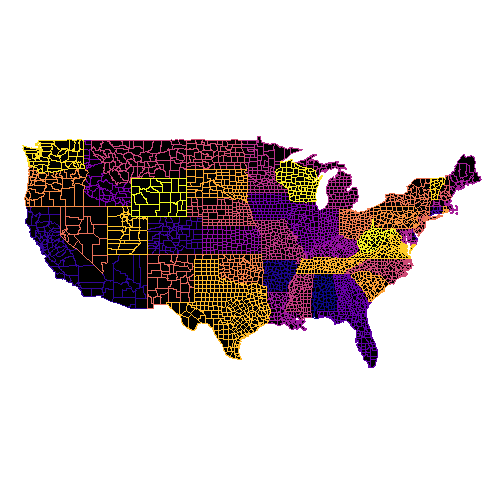
\includegraphics{final-models-proposed-county_level_files/figure-latex/unnamed-chunk-2-1.pdf}

\begin{Shaded}
\begin{Highlighting}[]
\NormalTok{county }\OperatorTok\StringTok{ }
\StringTok{  }\KeywordTok{drop_na}\NormalTok{() }\OperatorTok\StringTok{ }
\StringTok{  }\KeywordTok{group_by}\NormalTok{(year) }\OperatorTok\StringTok{ }
\StringTok{  }\KeywordTok{summarize}\NormalTok{(}\DataTypeTok{mean_percent =} \KeywordTok{mean}\NormalTok{(ltpa_percent)) }\OperatorTok\StringTok{ }
\StringTok{  }\KeywordTok{ggplot}\NormalTok{(}\KeywordTok{aes}\NormalTok{(year, mean_percent)) }\OperatorTok{+}
\StringTok{  }\KeywordTok{geom_line}\NormalTok{(}\DataTypeTok{color =} \StringTok{'dodgerblue'}\NormalTok{, }\DataTypeTok{size =} \DecValTok{1}\NormalTok{) }\OperatorTok{+}
\StringTok{  }\KeywordTok{geom_point}\NormalTok{() }\OperatorTok{+}
\StringTok{  }\KeywordTok{scale_y_continuous}\NormalTok{(}\DataTypeTok{name =} \StringTok{'Leisure-Time Physical Activity (%)'}\NormalTok{,}
                     \DataTypeTok{limits =} \KeywordTok{c}\NormalTok{(}\DecValTok{70}\NormalTok{, }\DecValTok{80}\NormalTok{))}
\end{Highlighting}
\end{Shaded}

\includegraphics{final-models-proposed-county_level_files/figure-latex/unnamed-chunk-2-2.pdf}

\begin{enumerate}
\def\labelenumi{\arabic{enumi}.}
\setcounter{enumi}{2}
\tightlist
\item
  Look into the role of percent latino
\end{enumerate}

\begin{Shaded}
\begin{Highlighting}[]
\KeywordTok{names}\NormalTok{(county)}
\end{Highlighting}
\end{Shaded}

\begin{verbatim}
##  [1] "rowid"                                         
##  [2] "state_fips_code"                               
##  [3] "county_fips_code"                              
##  [4] "fips_code"                                     
##  [5] "state"                                         
##  [6] "county_name"                                   
##  [7] "year"                                          
##  [8] "poor_or_fair_health"                           
##  [9] "poor_physical_health_days"                     
## [10] "poor_mental_health_days"                       
## [11] "adult_smoking"                                 
## [12] "adult_obesity"                                 
## [13] "food_environment_index"                        
## [14] "physical_inactivity"                           
## [15] "access_pa"                                     
## [16] "preventable_hospital_stays"                    
## [17] "some_college"                                  
## [18] "unemployment"                                  
## [19] "children_in_poverty"                           
## [20] "income_inequality"                             
## [21] "children_in_single_parent_households"          
## [22] "social_associations"                           
## [23] "violent_crime"                                 
## [24] "injury_deaths"                                 
## [25] "air_pollution_particulate_matter"              
## [26] "drinking_water_violations"                     
## [27] "severe_housing_problems"                       
## [28] "driving_alone_to_work"                         
## [29] "food_insecurity"                               
## [30] "limited_access_to_healthy_foods"               
## [31] "insufficient_sleep"                            
## [32] "uninsured_adults"                              
## [33] "uninsured_children"                            
## [34] "median_household_income"                       
## [35] "population"                                    
## [36] "percent_65_and_older"                          
## [37] "percent_asian"                                 
## [38] "percent_native_hawaiian_other_pacific_islander"
## [39] "percent_hispanic"                              
## [40] "percent_non_hispanic_white"                    
## [41] "percent_not_proficient_in_english"             
## [42] "percent_females"                               
## [43] "percent_rural"                                 
## [44] "phyact_percent"                                
## [45] "ltpa_percent"
\end{verbatim}

\begin{Shaded}
\begin{Highlighting}[]
\KeywordTok{describeBy}\NormalTok{(county}\OperatorTok{$}\NormalTok{percent_hispanic, }\DataTypeTok{group =}\NormalTok{ county}\OperatorTok{$}\NormalTok{year)}
\end{Highlighting}
\end{Shaded}

\begin{verbatim}
## 
##  Descriptive statistics by group 
## group: 2016
##    vars    n mean   sd median trimmed  mad min  max range skew kurtosis se
## X1    1 3191 0.09 0.13   0.04    0.06 0.03   0 0.96  0.96 3.12    11.29  0
## ------------------------------------------------------------ 
## group: 2017
##    vars    n mean   sd median trimmed  mad min  max range skew kurtosis se
## X1    1 3188 0.09 0.14   0.04    0.06 0.04   0 0.96  0.96 3.09    11.01  0
## ------------------------------------------------------------ 
## group: 2018
##    vars    n mean   sd median trimmed  mad  min  max range skew kurtosis se
## X1    1 3194 0.09 0.14   0.04    0.06 0.04 0.01 0.96  0.96 3.09    11.02  0
## ------------------------------------------------------------ 
## group: 2019
##    vars    n mean   sd median trimmed  mad  min  max range skew kurtosis se
## X1    1 3194  0.1 0.14   0.04    0.06 0.04 0.01 0.96  0.96 3.06    10.79  0
## ------------------------------------------------------------ 
## group: 2020
##    vars    n mean   sd median trimmed  mad  min  max range skew kurtosis se
## X1    1 3194  0.1 0.14   0.04    0.06 0.04 0.01 0.96  0.96 3.03    10.57  0
\end{verbatim}

\begin{Shaded}
\begin{Highlighting}[]
\NormalTok{county}\OperatorTok{$}\NormalTok{latino_group <-}\StringTok{ }\KeywordTok{cut}\NormalTok{(county}\OperatorTok{$}\NormalTok{percent_hispanic, }\DataTypeTok{breaks =} \DecValTok{3}\NormalTok{)}

\NormalTok{county }\OperatorTok\StringTok{ }
\StringTok{  }\KeywordTok{group_by}\NormalTok{(year) }\OperatorTok\StringTok{ }
\StringTok{  }\KeywordTok{count}\NormalTok{(latino_group)}
\end{Highlighting}
\end{Shaded}

\begin{verbatim}
## Warning: Factor `latino_group` contains implicit NA, consider using
## `forcats::fct_explicit_na`
\end{verbatim}

\begin{verbatim}
## # A tibble: 17 x 3
## # Groups:   year [6]
##     year latino_group        n
##    <dbl> <fct>           <int>
##  1  2016 (0.00102,0.323]  2984
##  2  2016 (0.323,0.643]     171
##  3  2016 (0.643,0.965]      36
##  4  2016 <NA>                2
##  5  2017 (0.00102,0.323]  2979
##  6  2017 (0.323,0.643]     172
##  7  2017 (0.643,0.965]      37
##  8  2018 (0.00102,0.323]  2982
##  9  2018 (0.323,0.643]     174
## 10  2018 (0.643,0.965]      38
## 11  2019 (0.00102,0.323]  2980
## 12  2019 (0.323,0.643]     173
## 13  2019 (0.643,0.965]      41
## 14  2020 (0.00102,0.323]  2978
## 15  2020 (0.323,0.643]     172
## 16  2020 (0.643,0.965]      44
## 17    NA <NA>                1
\end{verbatim}

\begin{Shaded}
\begin{Highlighting}[]
\NormalTok{county }\OperatorTok\StringTok{ }
\StringTok{  }\NormalTok{dplyr}\OperatorTok{::}\KeywordTok{select}\NormalTok{(year, percent_hispanic, access_pa, ltpa_percent, latino_group) }\OperatorTok\StringTok{ }
\StringTok{  }\KeywordTok{drop_na}\NormalTok{() }\OperatorTok\StringTok{ }
\StringTok{  }\KeywordTok{group_by}\NormalTok{(year) }\OperatorTok\StringTok{ }
\StringTok{  }\KeywordTok{mutate}\NormalTok{(}\DataTypeTok{access_percent =}\NormalTok{ access_pa}\OperatorTok{*}\DecValTok{100}\NormalTok{,}
         \DataTypeTok{latino_percent =}\NormalTok{ percent_hispanic}\OperatorTok{*}\DecValTok{100}\NormalTok{) }\OperatorTok
\StringTok{  }\KeywordTok{ggplot}\NormalTok{(}\KeywordTok{aes}\NormalTok{(access_percent, ltpa_percent)) }\OperatorTok{+}
\StringTok{  }\CommentTok{# geom_point(color = 'gray70', alpha = .9) + }
\StringTok{  }\KeywordTok{geom_smooth}\NormalTok{(}\DataTypeTok{method =} \StringTok{'lm'}\NormalTok{, }\DataTypeTok{se =} \OtherTok{FALSE}\NormalTok{, }\KeywordTok{aes}\NormalTok{(}\DataTypeTok{color =}\NormalTok{ latino_group)) }\OperatorTok{+}
\StringTok{  }\KeywordTok{facet_wrap}\NormalTok{(}\OperatorTok{~}\NormalTok{year)}
\end{Highlighting}
\end{Shaded}

\begin{verbatim}
## `geom_smooth()` using formula 'y ~ x'
\end{verbatim}

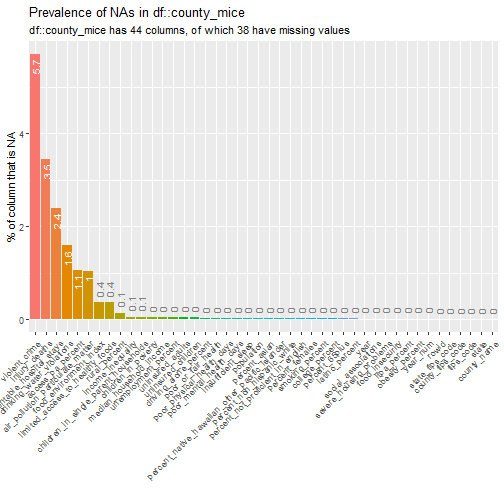
\includegraphics{final-models-proposed-county_level_files/figure-latex/unnamed-chunk-3-1.pdf}

\begin{enumerate}
\def\labelenumi{\arabic{enumi}.}
\setcounter{enumi}{2}
\item
  Z-score and make everything into percentages for analyses
\item
  Write out model equations.
\end{enumerate}

\begin{Shaded}
\begin{Highlighting}[]
\KeywordTok{names}\NormalTok{(county)}

\NormalTok{preliminary_ltpa_long <-}\StringTok{ }\KeywordTok{lmer}\NormalTok{(ltpa_percent }\OperatorTok{~}\StringTok{ }\NormalTok{year }\OperatorTok{+}\StringTok{ }\NormalTok{(}\DecValTok{1}\OperatorTok{|}\NormalTok{county_fips_code), }
                       \DataTypeTok{data =}\NormalTok{ county,}
                       \DataTypeTok{REML =} \OtherTok{FALSE}\NormalTok{,}
                    \DataTypeTok{control =} \KeywordTok{lmerControl}\NormalTok{(}\DataTypeTok{optimizer =} \StringTok{'Nelder_Mead'}\NormalTok{))}

\KeywordTok{summary}\NormalTok{(preliminary_ltpa_long)}

\KeywordTok{anova}\NormalTok{(preliminary_ltpa_long, preliminary_ltpa_long_}\DecValTok{3}\NormalTok{)}
\CommentTok{# physical activity over time (random effect of counties)}
\end{Highlighting}
\end{Shaded}

\[ Fixed Effect: LTPA_{ti} = \beta_{0i} + \beta_{1i}(year_{ti}) + \epsilon_{0ti} \]

\[ Random Effect: \beta_{0i} = \beta_0 + \mu_{0i}  \]

\[ Combined: LTPA_{ti} = \beta_0 + \beta_{1}(year_{ti}) + \mu_{0i}(year_{0ti}) + \epsilon_{0ti} \]

\[ Level 2: [\mu_{0i}] \sim N(0, \sigma^2_{\mu0}) \]

\[ Level 1: [\epsilon_{0ti}] \sim N(0,\sigma^2_{\epsilon0}) \]

\begin{Shaded}
\begin{Highlighting}[]
\NormalTok{preliminary_access_pa_long <-}\StringTok{ }\KeywordTok{lmer}\NormalTok{(access_pa }\OperatorTok{~}\StringTok{ }\NormalTok{year }\OperatorTok{+}\StringTok{ }\NormalTok{(}\DecValTok{1}\OperatorTok{|}\NormalTok{county_fips_code), }
                       \DataTypeTok{data =}\NormalTok{ county,}
                       \DataTypeTok{REML =} \OtherTok{FALSE}\NormalTok{,}
                    \DataTypeTok{control =} \KeywordTok{lmerControl}\NormalTok{(}\DataTypeTok{optimizer =} \StringTok{'Nelder_Mead'}\NormalTok{))}

\KeywordTok{summary}\NormalTok{(preliminary_access_pa_long)}

\KeywordTok{anova}\NormalTok{(preliminary_access_pa_long, preliminary_access_pa_long_}\DecValTok{3}\NormalTok{)}
\CommentTok{# access to physical activity over time (random effect of counties)}
\end{Highlighting}
\end{Shaded}

\[ Fixed Effect: AccessPA_{ti} = \beta_{0i} + \beta_{1i}(year_{ti}) + \epsilon_{0ti} \]

\[ Random Effect: \beta_{0i} = \beta_0 + \mu_{0i}  \]

\[ Combined: AccessPA_{ti} = \beta_0 + \beta_{1}(year_{ti}) + \mu_{0i}(year_{0ti}) + \epsilon_{0ti} \]

\[ Level 2: [\mu_{0i}] \sim N(0, \sigma^2_{\mu0}) \]

\[ Level 1: [\epsilon_{0ti}] \sim N(0,\sigma^2_{\epsilon0}) \]

\begin{Shaded}
\begin{Highlighting}[]
\KeywordTok{names}\NormalTok{(county)}

\NormalTok{ltpa_long_controls <-}\StringTok{ }\KeywordTok{lmer}\NormalTok{(ltpa_percent }\OperatorTok{~}\StringTok{ }\NormalTok{year }\OperatorTok{+}\StringTok{ }\NormalTok{violent_crime }\OperatorTok{+}
\StringTok{                                  }\NormalTok{adult_obesity }\OperatorTok{+}\StringTok{ }\NormalTok{some_college }\OperatorTok{+}
\StringTok{                                  }\NormalTok{income_inequality }\OperatorTok{+}\StringTok{ }\NormalTok{air_pollution_particulate_matter }\OperatorTok{+}
\StringTok{                                  }\NormalTok{driving_alone_to_work }\OperatorTok{+}\StringTok{ }\NormalTok{percent_rural }\OperatorTok{+}
\StringTok{                                  }\NormalTok{(}\DecValTok{1}\OperatorTok{|}\NormalTok{county_fips_code), }
                       \DataTypeTok{data =}\NormalTok{ county,}
                       \DataTypeTok{REML =} \OtherTok{FALSE}\NormalTok{,}
                    \DataTypeTok{control =} \KeywordTok{lmerControl}\NormalTok{(}\DataTypeTok{optimizer =} \StringTok{'Nelder_Mead'}\NormalTok{))}

\KeywordTok{summary}\NormalTok{(ltpa_long_controls)}


\KeywordTok{anova}\NormalTok{(preliminary_ltpa_long, ltpa_long_controls)}
\end{Highlighting}
\end{Shaded}

\[ Fixed Effect: AccessPA_{ti} = \beta_{0i} + \beta_{1i}(Year_{ti}) + \beta_{2i}(ViolentCrime_{ti})+ \beta_{3i}(Obesity_{ti}) + \beta_{4i}(SomeCollege_{ti}) + \beta_{5i}(IncomeInequality_{ti}) + \beta_{6i}(AirPollution_{ti}) + \beta_{7i}(DrivingAlone_{ti}) + \beta_{8i}(Rurality_{ti}) + \epsilon_{0ti} \]

\[ Random Effect: \beta_{0i} = \beta_0 + \mu_{0i}  \]

\[ Combined: AccessPA_{ti} = \beta_0 + \beta_{1}(year_{ti}) + \beta_{2}(ViolentCrime_{ti})+ \beta_{3}(Obesity_{ti}) + \beta_{4}(SomeCollege_{ti}) + \beta_{5}(IncomeInequality_{ti}) + \beta_{6}(AirPollution_{ti}) + \beta_{7}(DrivingAlone_{ti}) + \beta_{8}(Rurality_{ti}) + \mu_{0i}(year_{0ti}) + \epsilon_{0ti} \]

\[ Level 2: [\mu_{0i}] \sim N(0, \sigma^2_{\mu0}) \]

\[ Level 1: [\epsilon_{0ti}] \sim N(0,\sigma^2_{\epsilon0}) \]

\begin{Shaded}
\begin{Highlighting}[]
\NormalTok{ltpa_long_access <-}\StringTok{ }\KeywordTok{lmer}\NormalTok{(ltpa_percent }\OperatorTok{~}\StringTok{ }\NormalTok{year }\OperatorTok{+}\StringTok{ }\NormalTok{violent_crime }\OperatorTok{+}
\StringTok{                                  }\NormalTok{adult_obesity }\OperatorTok{+}\StringTok{ }\NormalTok{some_college }\OperatorTok{+}
\StringTok{                                  }\NormalTok{income_inequality }\OperatorTok{+}\StringTok{ }\NormalTok{air_pollution_particulate_matter }\OperatorTok{+}
\StringTok{                                  }\NormalTok{driving_alone_to_work }\OperatorTok{+}\StringTok{ }\NormalTok{percent_rural }\OperatorTok{+}\StringTok{ }
\StringTok{                                  }\NormalTok{access_pa }\OperatorTok{+}\StringTok{ }\NormalTok{(}\DecValTok{1}\OperatorTok{|}\NormalTok{county_fips_code), }
                       \DataTypeTok{data =}\NormalTok{ county,}
                       \DataTypeTok{REML =} \OtherTok{FALSE}\NormalTok{,}
                    \DataTypeTok{control =} \KeywordTok{lmerControl}\NormalTok{(}\DataTypeTok{optimizer =} \StringTok{'Nelder_Mead'}\NormalTok{))}

\KeywordTok{summary}\NormalTok{(ltpa_long_access)}

\KeywordTok{anova}\NormalTok{(ltpa_long_controls, ltpa_long_access)}
\end{Highlighting}
\end{Shaded}

\[ Fixed Effect: AccessPA_{ti} = \beta_{0i} + \beta_{1i}(Year_{ti}) + \beta_{2i}(ViolentCrime_{ti})+ \beta_{3i}(Obesity_{ti}) + \beta_{4i}(SomeCollege_{ti}) + \beta_{5i}(IncomeInequality_{ti}) + \beta_{6i}(AirPollution_{ti}) + \beta_{7i}(DrivingAlone_{ti}) + \beta_{8i}(Rurality_{ti}) + \beta_{9i}(LTPA_{ti}) + \epsilon_{0ti} \]

\[ Random Effect: \beta_{0i} = \beta_0 + \mu_{0i}  \]

\[ Combined: AccessPA_{ti} = \beta_0 + \beta_{1}(year_{ti}) + \beta_{2}(ViolentCrime_{ti})+ \beta_{3}(Obesity_{ti}) + \beta_{4}(SomeCollege_{ti}) + \beta_{5}(IncomeInequality_{ti}) + \beta_{6}(AirPollution_{ti}) + \beta_{7}(DrivingAlone_{ti}) + \beta_{8}(Rurality_{ti}) + \beta_{9}(LTPA_{ti}) + \mu_{0i}(year_{0ti}) + \epsilon_{0ti} \]

\[ Level 2: [\mu_{0i}] \sim N(0, \sigma^2_{\mu0}) \]

\[ Level 1: [\epsilon_{0ti}] \sim N(0,\sigma^2_{\epsilon0}) \]

\begin{Shaded}
\begin{Highlighting}[]
\NormalTok{access_latino_int <-}\StringTok{ }\KeywordTok{lmer}\NormalTok{(ltpa_percent }\OperatorTok{~}\StringTok{ }\NormalTok{year }\OperatorTok{+}\StringTok{ }\NormalTok{violent_crime }\OperatorTok{+}
\StringTok{                                  }\NormalTok{adult_obesity }\OperatorTok{+}\StringTok{ }\NormalTok{some_college }\OperatorTok{+}
\StringTok{                                  }\NormalTok{income_inequality }\OperatorTok{+}\StringTok{ }\NormalTok{air_pollution_particulate_matter }\OperatorTok{+}
\StringTok{                                  }\NormalTok{driving_alone_to_work }\OperatorTok{+}\StringTok{ }\NormalTok{percent_rural }\OperatorTok{+}\StringTok{ }
\StringTok{                                  }\NormalTok{access_pa}\OperatorTok{*}\NormalTok{percent_hispanic }\OperatorTok{+}\StringTok{ }\NormalTok{(}\DecValTok{1}\OperatorTok{|}\NormalTok{county_fips_code), }
                       \DataTypeTok{data =}\NormalTok{ county,}
                       \DataTypeTok{REML =} \OtherTok{FALSE}\NormalTok{,}
                    \DataTypeTok{control =} \KeywordTok{lmerControl}\NormalTok{(}\DataTypeTok{optimizer =} \StringTok{'Nelder_Mead'}\NormalTok{))}

\KeywordTok{summary}\NormalTok{(access_latino_int)}


\KeywordTok{anova}\NormalTok{(ltpa_long_access, access_latino_int)}
\end{Highlighting}
\end{Shaded}

\[ Fixed Effect: AccessPA_{ti} = \beta_{0i} + \beta_{1i}(Year_{ti}) + \beta_{2i}(ViolentCrime_{ti})+ \beta_{3i}(Obesity_{ti}) + \beta_{4i}(SomeCollege_{ti}) + \beta_{5i}(IncomeInequality_{ti}) + \beta_{6i}(AirPollution_{ti}) + \beta_{7i}(DrivingAlone_{ti}) + \beta_{8i}(Rurality_{ti}) + \beta_{9i}(LTPA_{ti}) + \beta_{10i}(LatinoPercent_{ti}) + \beta_{11i}(LTPA*LatinoPercent_{ti}) + \epsilon_{0ti} \]

\[ Random Effect: \beta_{0i} = \beta_0 + \mu_{0i}  \]

\[ Combined: AccessPA_{ti} = \beta_0 + \beta_{1}(year_{ti}) + \beta_{2}(ViolentCrime_{ti})+ \beta_{3}(Obesity_{ti}) + \beta_{4}(SomeCollege_{ti}) + \beta_{5}(IncomeInequality_{ti}) + \beta_{6}(AirPollution_{ti}) + \beta_{7}(DrivingAlone_{ti}) + \beta_{8}(Rurality_{ti}) + \beta_{9}(LTPA_{ti}) + \beta_{10}(LatinoPercent_{ti}) + \beta_{11}(LTPA*LatinoPercent_{ti}) + \mu_{0i}(year_{0ti}) + \epsilon_{0ti} \]

\[ Level 2: [\mu_{0i}] \sim N(0, \sigma^2_{\mu0}) \]

\[ Level 1: [\epsilon_{0ti}] \sim N(0,\sigma^2_{\epsilon0}) \]

\begin{enumerate}
\def\labelenumi{\arabic{enumi}.}
\setcounter{enumi}{4}
\tightlist
\item
  Look into times for multiple imputations, since there is over 5\% of
  missing data for
\end{enumerate}

\end{document}
